\appendix
\clearpage
\section{Appendix}
\label{sec:appendix}

\begin{figure}[h]
	\centering
	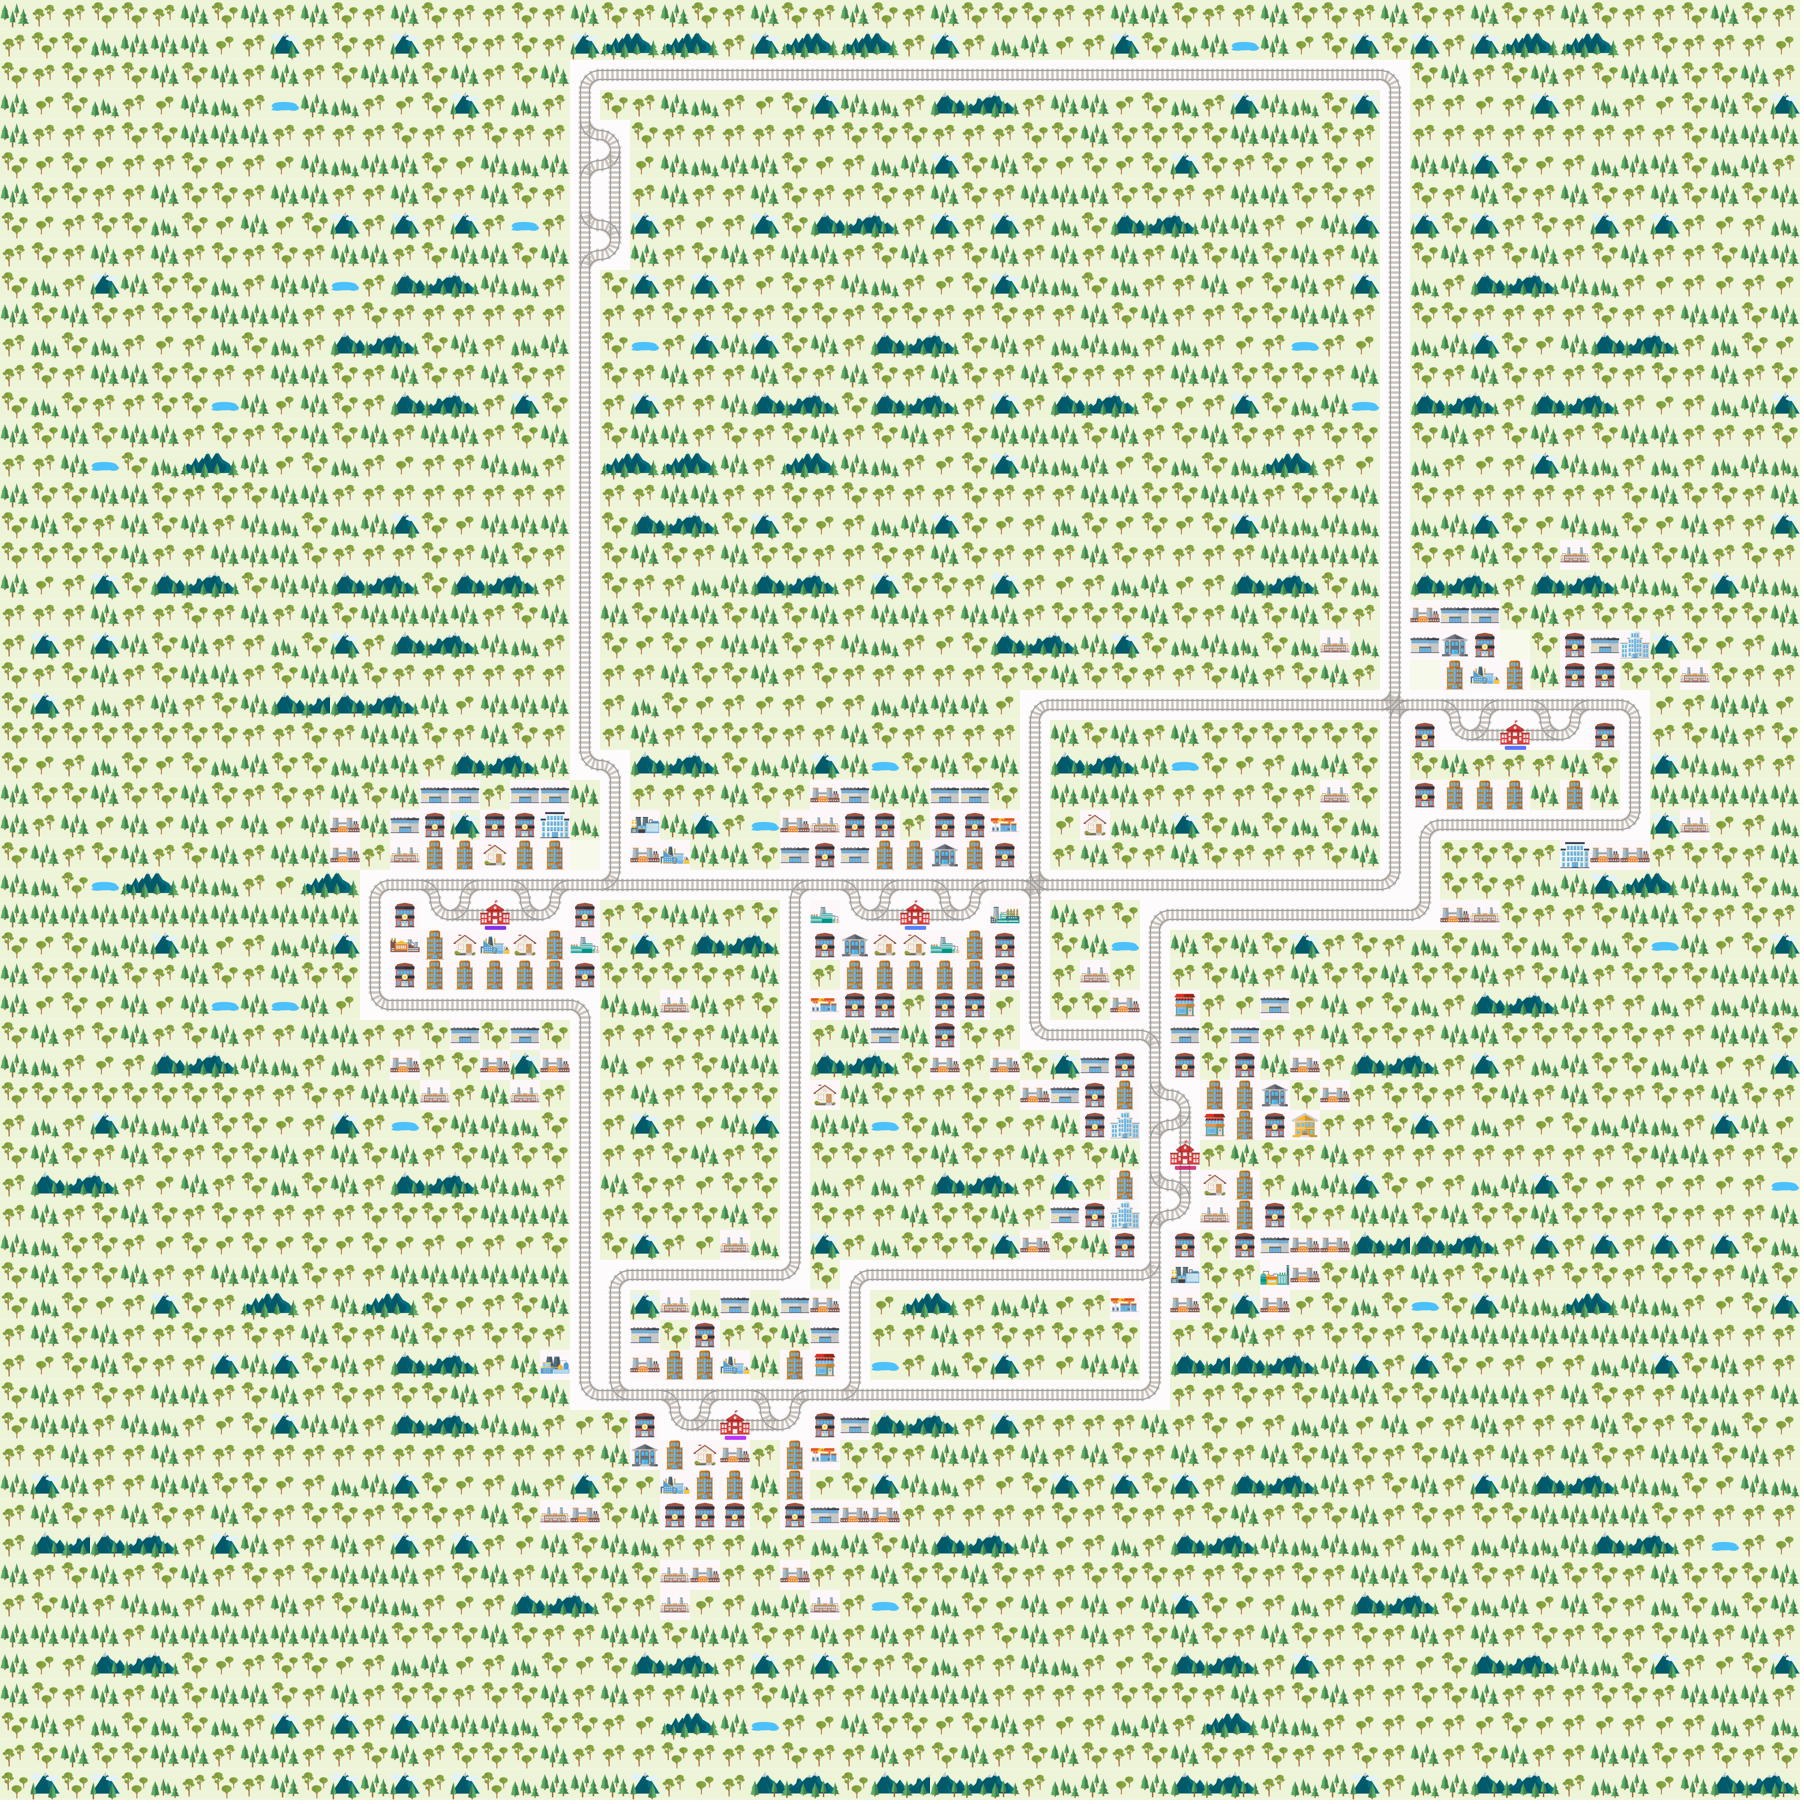
\includegraphics[width=0.9\textwidth]{sparse/sparse_0_1}
	\caption{Sparse instance, using a 60x60 grid, where 6 trains must travel across 6 cities.}
	\label{sparse_0_1_fullpage}
\end{figure}

\begin{figure}[h]
	\centering
	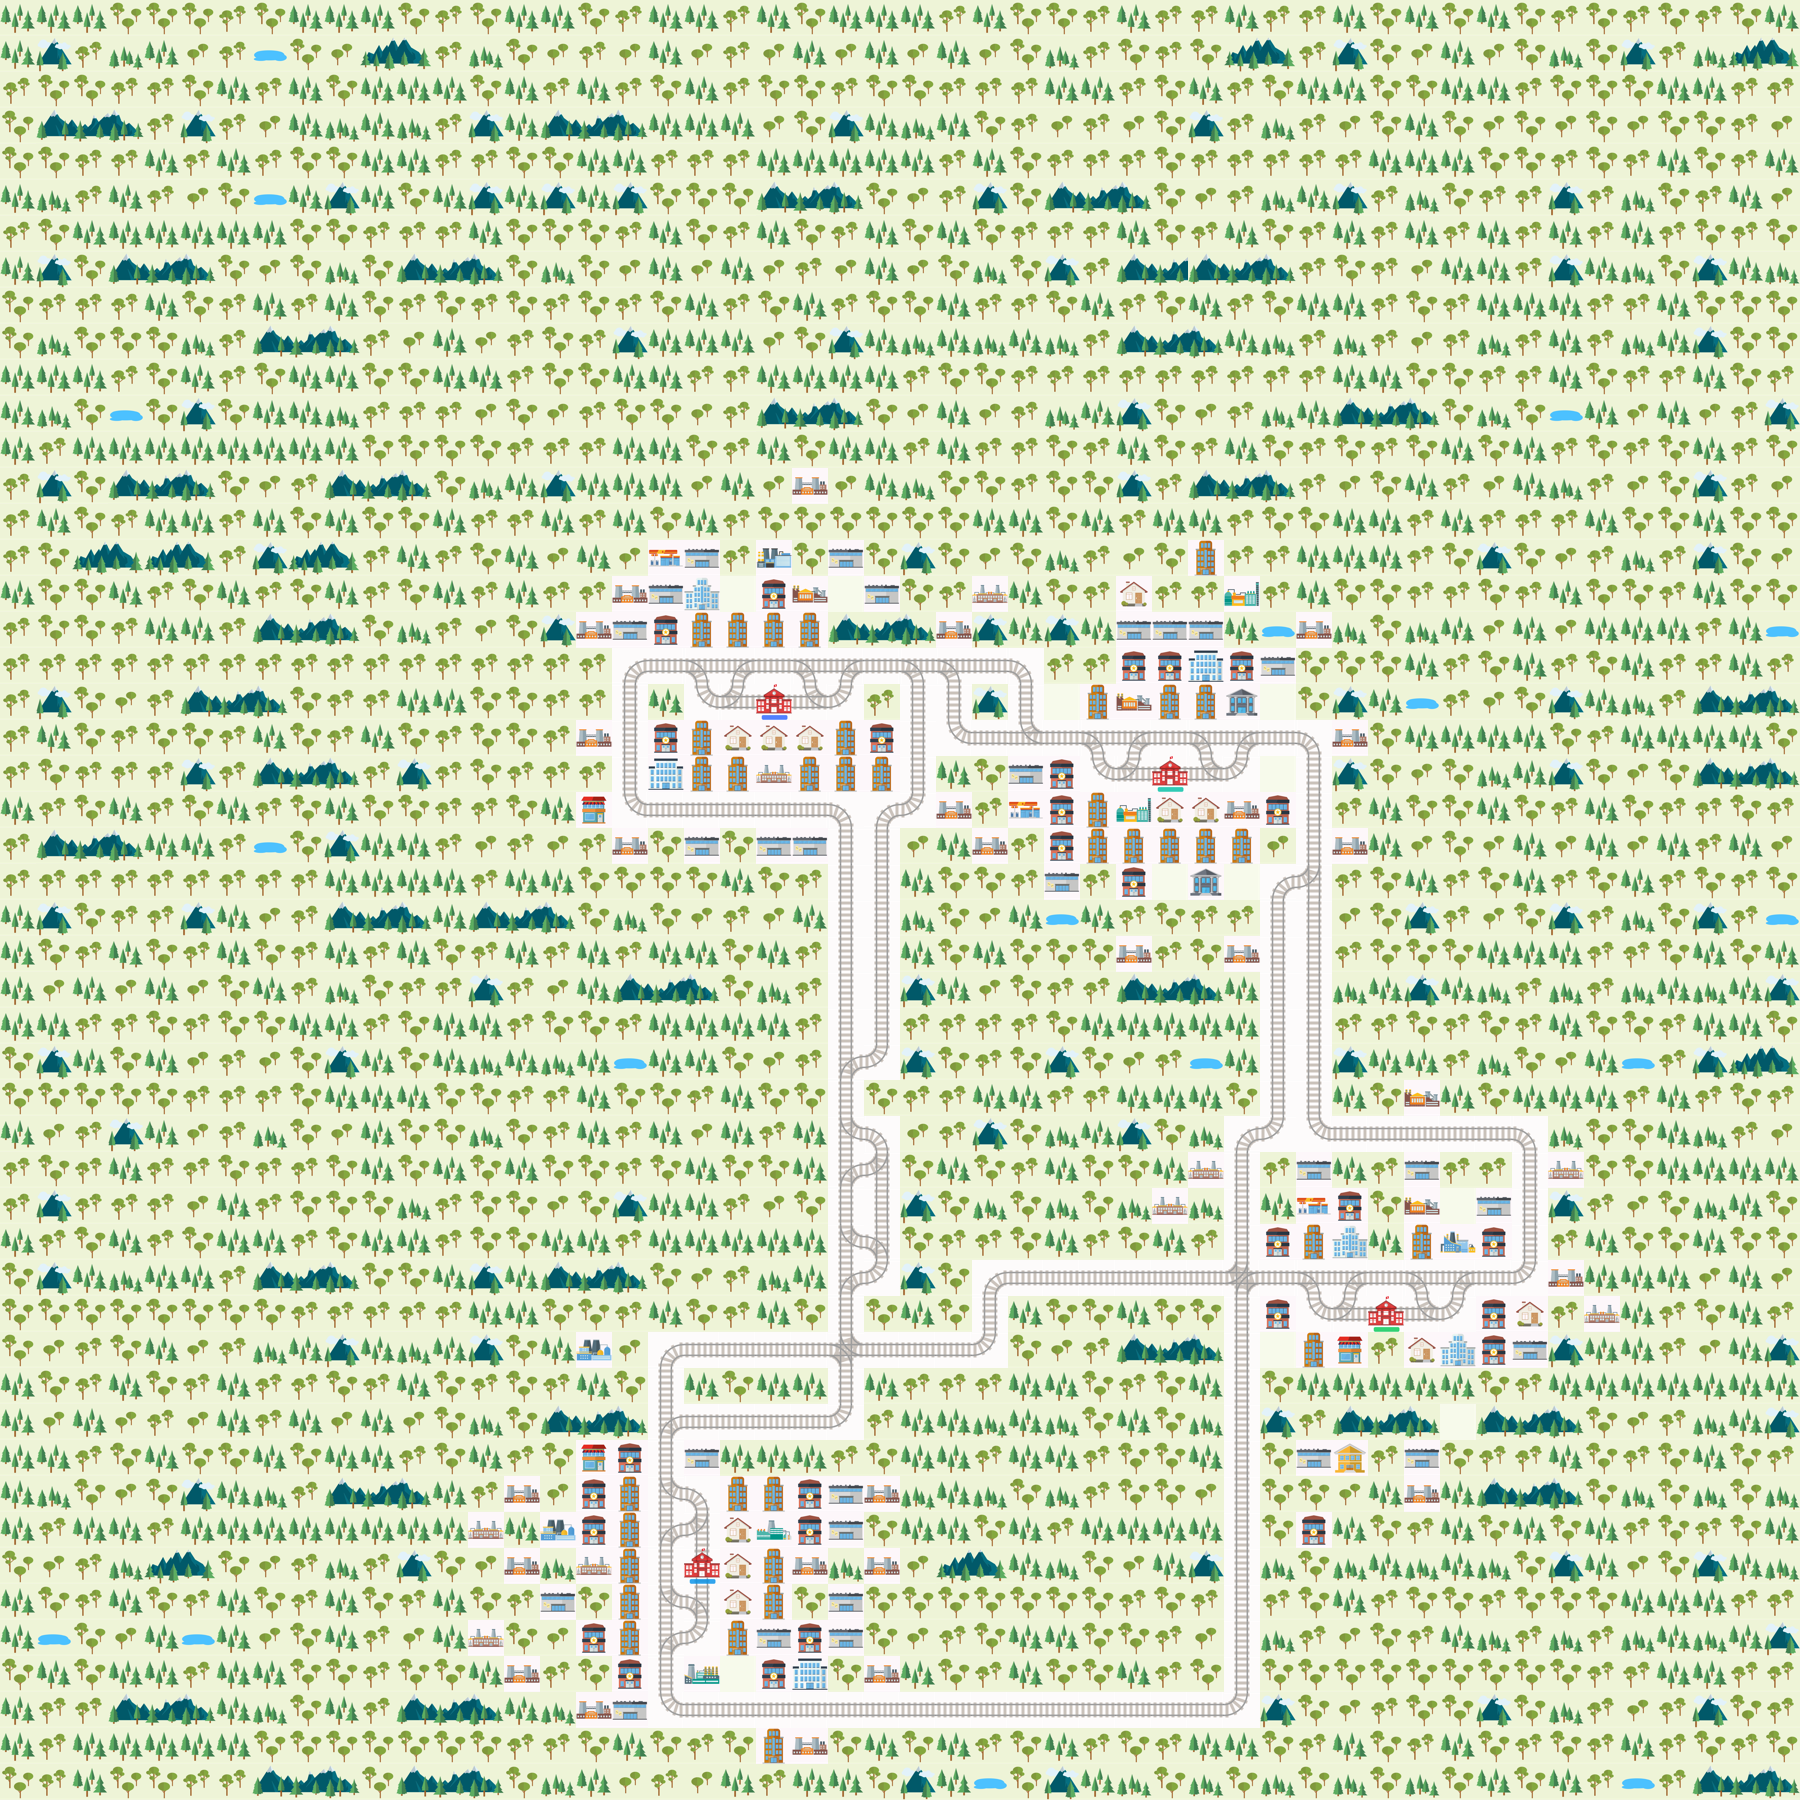
\includegraphics[width=0.9\textwidth]{medium/medium_0_1}
	\caption{Medium instance, using a 50x50 grid, where 10 trains must travel across 5 cities.}
	\label{medium_0_1_fullpage}
\end{figure}

\begin{figure}[h]
	\centering
	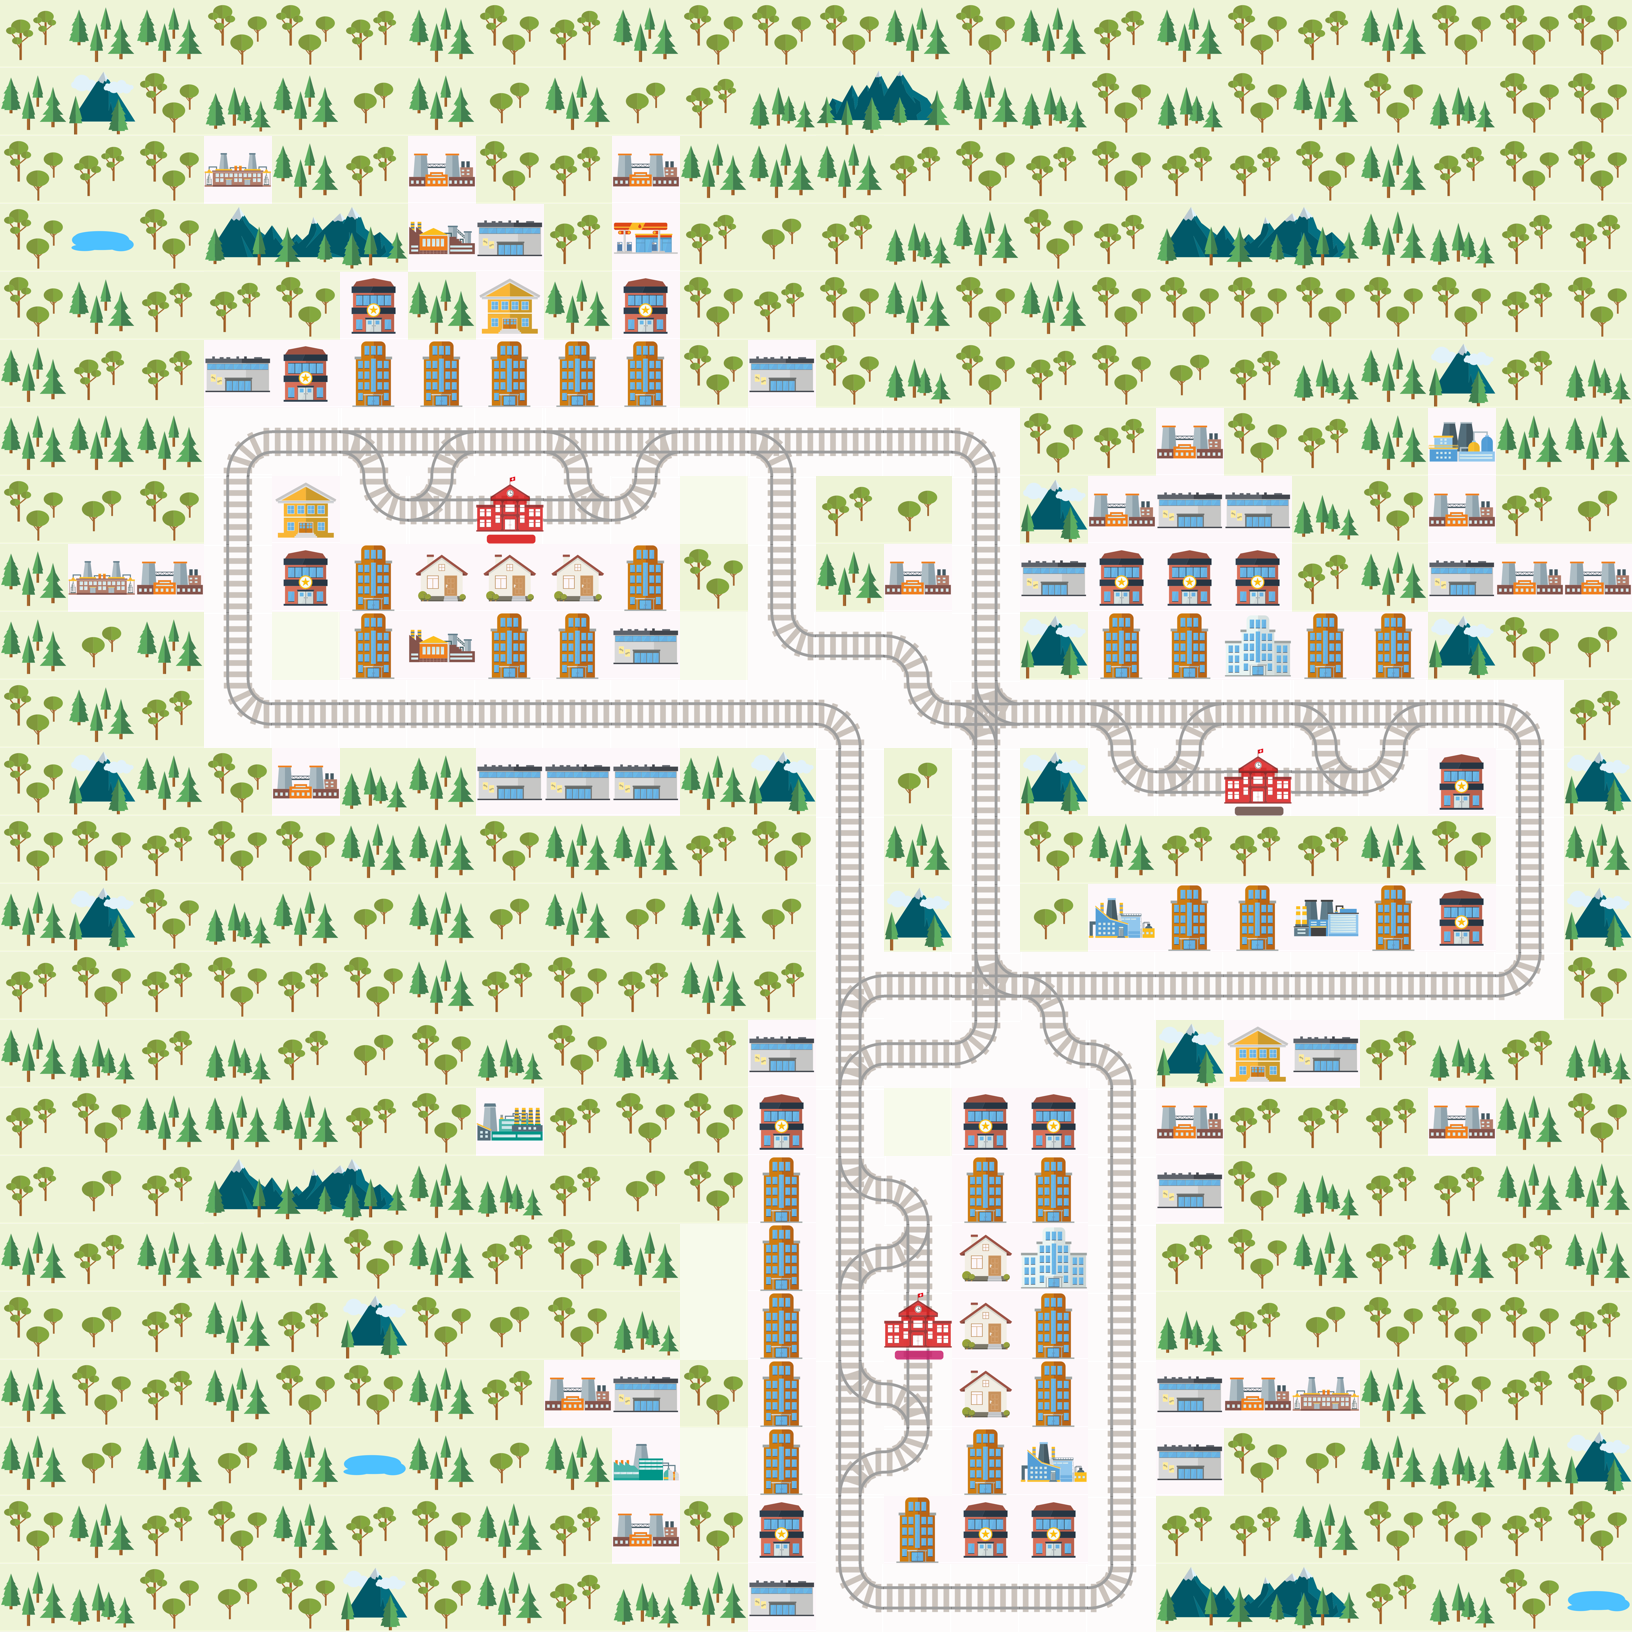
\includegraphics[width=0.9\textwidth]{dense/dense_0_1}
	\caption{Dense instance, using a 24x24 grid, where 20 trains must travel across 3 cities.}
	\label{dense_0_1_fullpage}
\end{figure}

\begin{figure}[h]
	\centering
	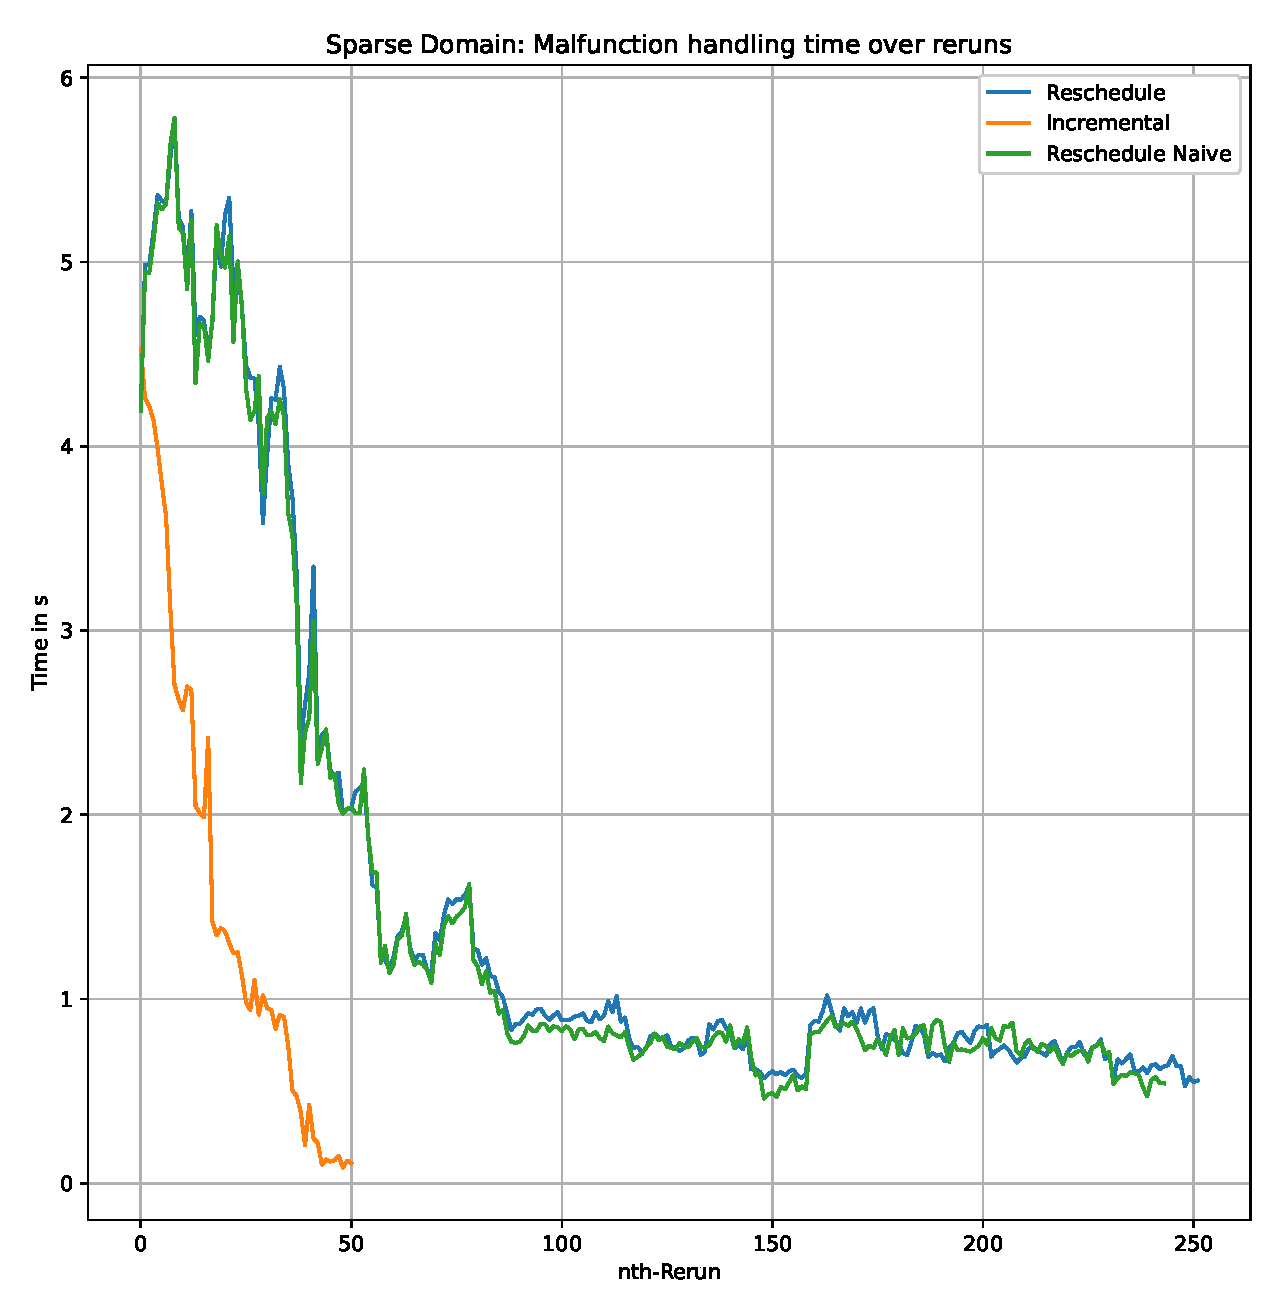
\includegraphics[width=0.9\textwidth]{benchmarking/sparse_rerun_full.eps}
	\caption{Full Sparse Benchmark}
	\label{dense_0_1_fullpage}
\end{figure}

\begin{figure}[h]
	\centering
	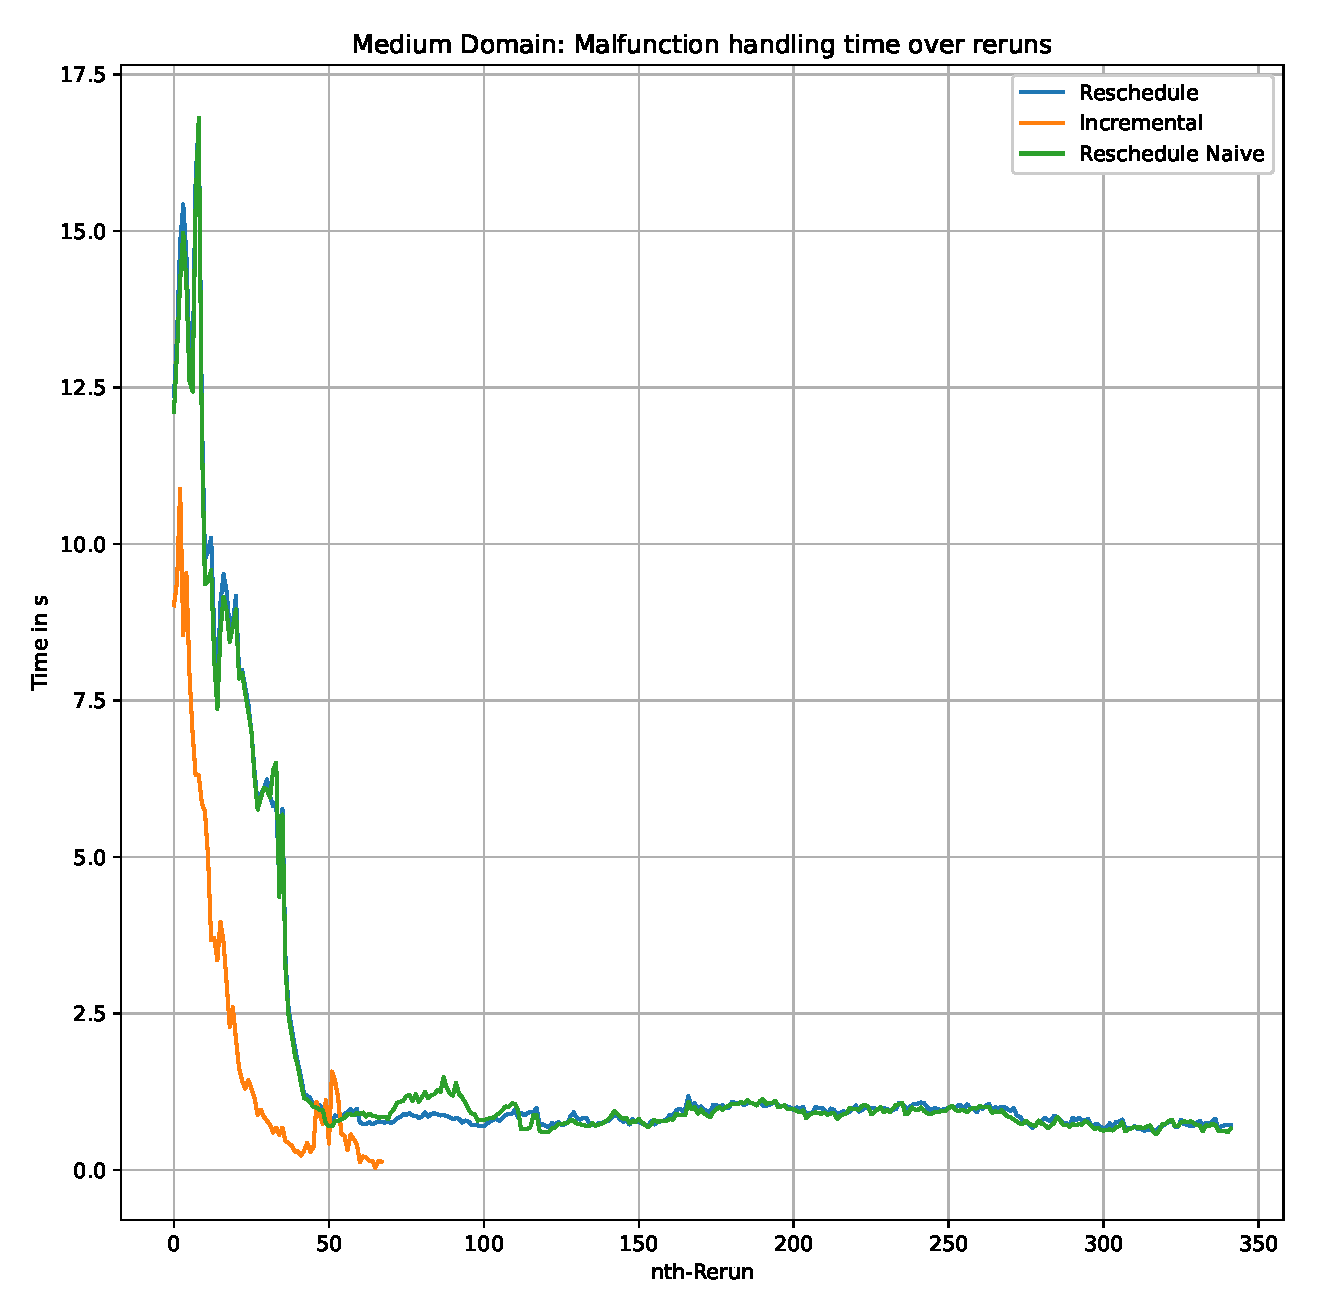
\includegraphics[width=0.9\textwidth]{benchmarking/medium_rerun_full.eps}
	\caption{Full Medium Benchmark}
	\label{dense_0_1_fullpage}
\end{figure}

\begin{figure}[h]
	\centering
	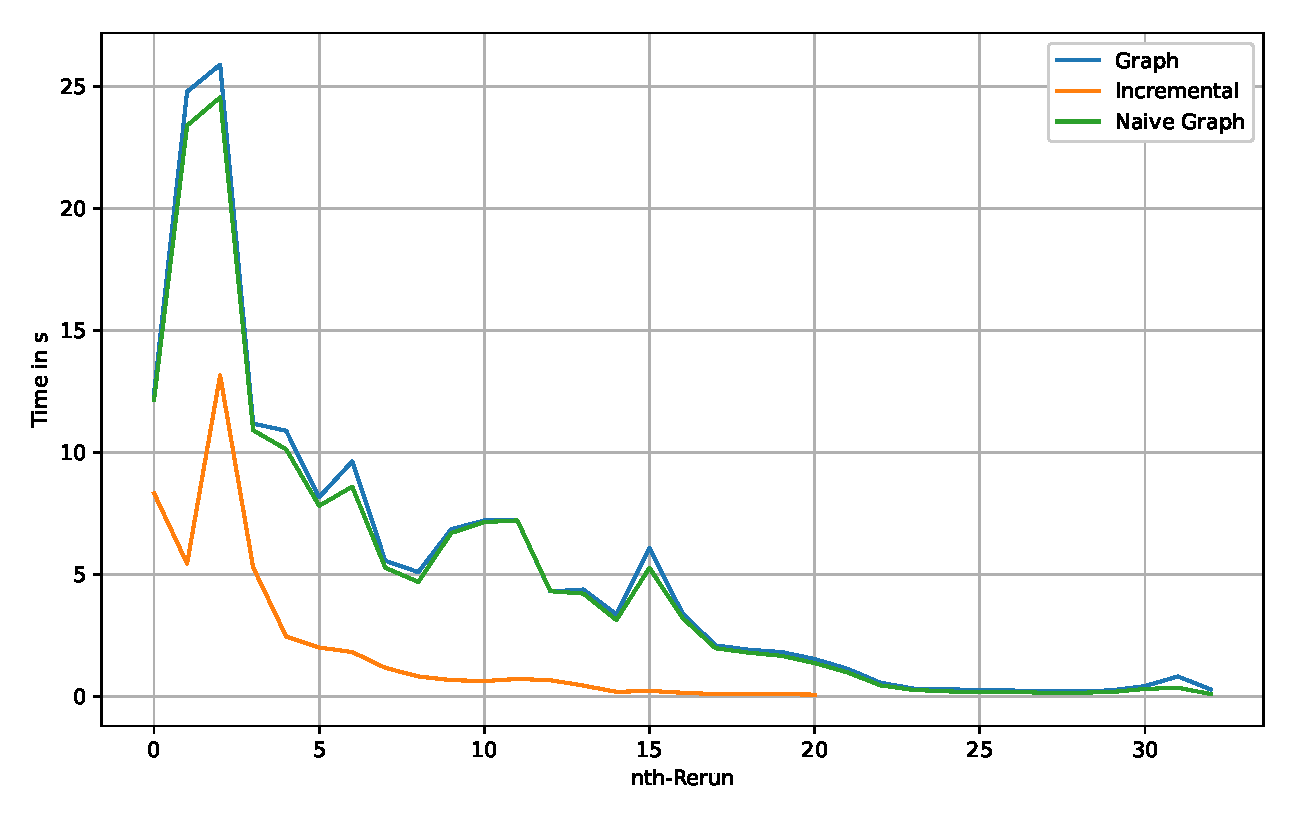
\includegraphics[width=0.9\textwidth]{benchmarking/dense_rerun_full.eps}
	\caption{Full Dense Benchmark}
	\label{dense_0_1_fullpage}
\end{figure}